\chapter{Multiple sediment fractions -- proof of concept}

To test the implementation of the sediment class formulation a comparison is made with observations of pre-and post hurricane Ivan cross-barrier island profiles (see Figure 6.1) at Beasly Park, Florida, USA \citep{WangHorwitz2007}. 

The hurricane Ivan impact is simulated with a constant surge level of \textit{1.8 }m present for \textit{10} hours at which time the offshore incident significant wave height is kept at \textit{10} m with a mean wave period of 12 s. The sediment class distribution used in the calculations discriminates between sand located within the frontal dune (class 1) and sand located on and behind the barrier island (class 2) (see upper panel in ). The sand on the barrier island is mostly vegetated which mitigates the erosion. Hence this sand has been given a mobility restriction that makes it more difficult to pick-up by means of a reduction factor of \textit{0.25} on the equilibrium concentration. Grain sizes for both sand composites are the same with a D${}_{50}$${}_{ }$of 0.0035 m and a D${}_{90}$${}_{ }$of 0.005 mm. The initial sediment class distribution is presented in the top panel of Figure 1, where an intensity of 1 corresponds to sediment class one only and -1 to the presence of sediment class 2 only.  

The bed-elevation and sediment class distribution after 10 hours are shown in the lower panel of . The calculated bed-level is similar to the observations although differences are apparent. These differences can be related to the fact that the hurricane impact is simply modeled (i.e. constant conditions) and the fact that the post-survey was performed approximately 10 months after the hurricane had past. Still the overall evolution is consistent with the observations. The calculated changes in the sediment classes are also consistent with the observations of \citet{WangHorwitz2007} based on a number of cores showing that the intersection of the new washover with the pre-hurricane sediment occurs approximately at the original bed level.

\begin{figure}[h]
  \centering
  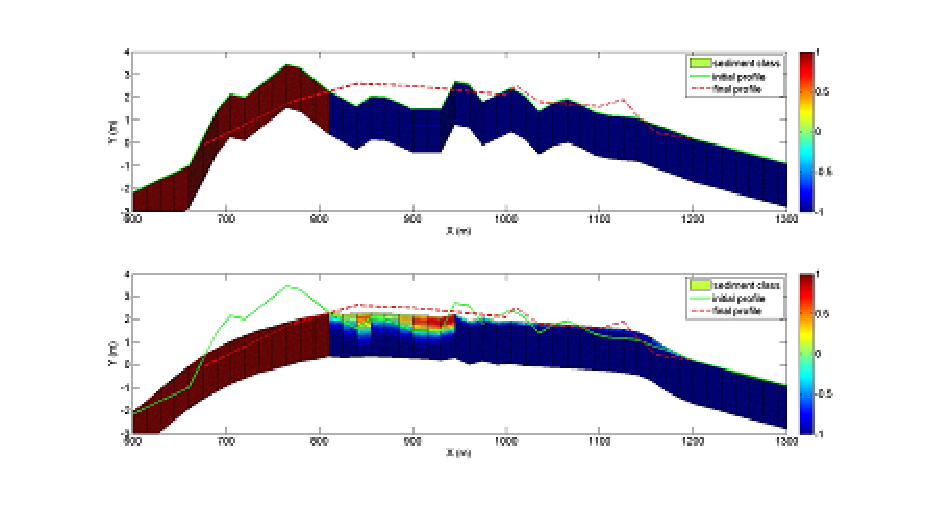
\includegraphics[width=\textwidth]{image46}
  \caption{Top panel: Initial pre-hurricane bed elevation (green line) and sediment class distribution. A value of 1 corresponds to 100\% of sediment class 1, a value of 0 to 50\% of class 1 and 50 \% of class 2, and a value of -1 corresponds to 100 \% of sediment class two. Post-hurricane bed elevation (dashed red line) given as a reference. Bottom panel: Calculated bed-evolution (corresponding to the position of the top layer) and corresponding sediment class distribution showing the thickness of the wash-over layer located behind the initial dune. Pre- (green line) and post-hurricane (red dashed line) bed elevation given as a reference}
  \label{fig:image46}
\end{figure}

%%% Local Variables: 
%%% mode: latex
%%% TeX-master: "xbeach_manual"
%%% End: 
